%%
%% ICAIF 2026 Submission — v6: cost-speed frontier narrative
%% ACM Conference Proceedings Format
%%
\documentclass[sigconf,review,anonymous,balance=false]{acmart}

%% Rights management information
\setcopyright{acmlicensed}
\copyrightyear{2026}
\acmYear{2026}
\acmDOI{}

%% Conference information
\acmConference[ICAIF '26]{7th ACM International Conference on AI in Finance}{November 14--17, 2026}{Milan, Italy}
\acmBooktitle{Proceedings of the 7th ACM International Conference on AI in Finance (ICAIF '26), November 14--17, 2026, Milan, Italy}
\acmISBN{}

%% Packages
\usepackage{booktabs}
\usepackage{amsmath}
\usepackage{subcaption}
\usepackage{xcolor}
\usepackage{graphicx}

%% Allow modest interword stretch to avoid overfull lines
\emergencystretch=1.5em

%%
%% end of the preamble, start of the body of the document source.
\begin{document}

%%
%% Title
\title{Feature Speed, Transaction Costs, and the Limits of Machine Learning in Emerging Markets}

%%
%% Authors
\author{Anonymous Author(s)}
\affiliation{%
  \institution{Anonymous Institution}
  \city{Anonymous City}
  \country{Anonymous Country}
}
\email{anonymous@anonymous.com}

%%
%% Abstract
\begin{abstract}
Across 15 emerging markets, eight portfolio interventions
converge on the same net Sharpe ceiling (${\sim}$0.45--0.49 at
3$\times$ transaction costs), regardless of whether they restrict
features, smooth predictions, or reduce
rebalancing frequency. We show this ceiling is traced by a
cost-speed frontier: $\text{SR}_{\text{gross}} - \text{SR}_{\text{net}}
\approx \lambda \kappa \cdot \text{FSI} + c$, where the Feature Speed
Index (FSI) measures a strategy's ex-ante exposure to fast-moving
characteristics. FSI explains 64--65\% of cross-sectional SR
degradation at each cost level ($\lambda = 0.33$ per unit $\kappa$;
pooled $R^2 = 0.72$ across 300 strategy--market--cost combinations)
and predicts realized turnover ex ante ($R^2 = 0.73$).
Non-smooth models (trees, neural networks) fall systematically below
the frontier, revealing model smoothness as a second constraint.
The frontier explains why ML's prediction advantage (gross SR 0.68 vs.\
sorts' 0.58) vanishes after costs: ML loads on fast features that
generate 2--3$\times$ the turnover of sorts. Restricting Ridge regression to
slow, persistent characteristics is the simplest path to the ceiling
(SR 0.47, 10\% turnover); EMA smoothing and quarterly rebalancing
reach the same frontier through different mechanisms, while cost-aware
neural networks trade away signal for turnover and fall short.
\end{abstract}

%%
%% CCS Concepts
\begin{CCSXML}
<ccs2012>
<concept>
<concept_id>10002950.10003648.10003688</concept_id>
<concept_desc>Mathematics of computing~Probabilistic algorithms</concept_desc>
<concept_significance>500</concept_significance>
</concept>
<concept>
<concept_id>10010147.10010257</concept_id>
<concept_desc>Computing methodologies~Machine learning</concept_desc>
<concept_significance>500</concept_significance>
</concept>
</ccs2012>
\end{CCSXML}

\ccsdesc[500]{Mathematics of computing~Probabilistic algorithms}
\ccsdesc[500]{Computing methodologies~Machine learning}

%%
%% Keywords
\keywords{machine learning, emerging markets, transaction costs, portfolio construction, factor investing}

%%
%% Maketitle
\maketitle


%% ===================================================================
%% 1. INTRODUCTION
%% ===================================================================
\section{Introduction}

Machine learning has transformed cross-sectional asset pricing. Gu,
Kelly, and Xiu~\cite{gu2020empirical} show that tree-based and neural
network models produce superior out-of-sample $R^2$ for US equities,
and Hanauer and Kalsbach~\cite{hanauer2023machine} extend this to
emerging markets (EM). More recently, Jensen, Kelly, Malamud, and
Pedersen~\cite{jensen2024implementable} (JKMP) identify that
cost-agnostic ML overweights ``fleeting small-scale characteristics,''
proposing an ``implementable efficient frontier'' that integrates costs
into the optimization objective.

We build on their diagnosis and show that the cost--speed interaction
creates a \emph{performance ceiling}: across 15 emerging markets, eight
intervention variants spanning four mechanism families (feature
selection, persistence filtering,
prediction smoothing, quarterly rebalancing) all converge on
net SR ${\sim}$0.45--0.49 at 3$\times$ EM costs. Where JKMP optimize
toward an implementable frontier, we characterize the ceiling that any
method (upstream or downstream) approaches, and provide an ex-ante
diagnostic, the Feature Speed Index (FSI), computable from training
data alone. Our central contribution is the frontier as an ex-ante
diagnostic: FSI, computed from training data alone, explains 64--65\%
of cross-sectional cost-driven SR degradation at every cost level
and 73\% of realized turnover.

Five findings anchor the analysis, using 154 firm-level
characteristics from the JKP Global Factor
Data~\cite{JensenKellyPedersen2023}, walk-forward validation, and
Corwin-Schultz~\cite{corwinschultz2012} transaction costs:

\begin{enumerate}
    \item \textbf{A cost-speed ceiling.} Eight intervention variants
    converge on net SR ${\sim}$0.45--0.49 despite different mechanisms.
    The frontier $\text{SR}_{\text{gross}} - \text{SR}_{\text{net}}
    \approx \lambda\kappa \cdot \text{FSI} + c$ fits SR degradation
    with pooled $R^2 = 0.72$ across 300 strategy--market--cost
    combinations; at each fixed cost level, FSI explains 64--65\% of
    cross-sectional degradation ($\lambda = 0.33$ per unit $\kappa$).

    \item \textbf{Cost--speed interaction.} At zero costs, fast and slow
    features produce comparable gross SRs (0.63 vs.\ 0.61). At
    3$\times$ EM costs, fast features degrade ${\sim}3\times$ faster
    (SR degradation 0.42 vs.\ 0.14).

    \item \textbf{Simple upstream fixes reach the ceiling.} Restricting
    Ridge to slow features (57 characteristics) achieves net SR 0.47
    at 10\% turnover vs.\ standard Ridge (0.35, 23\%) and MomentumSort
    (0.36, 17\%), outperforming the sort in 11/15 markets (not
    individually significant; Section~\ref{sec:robustness}).

    \item \textbf{ML overweights fast features.} ML allocates
    43--47\% of importance to fast features (25\% of the set),
    driving 63\% of prediction changes.

    \item \textbf{Prediction stability is the binding constraint.}
    Tree models pair the strongest gross signals with the worst net
    SRs (XGBoost 0.66 gross, 0.17 net; Table~\ref{tab:gross_vs_net})
    and slow features do not help; walk-forward EMA smoothing lifts
    XGBoost only to sort parity (0.35), not to the frontier.
    Prediction stability, not accuracy, is the binding constraint.
\end{enumerate}

A cross-regime validation on US equities (top 500, 2021--2025) confirms
the decomposition: Ridge\_Slow outperforms Ridge\_Fast at every cost
level, and Ridge\_Fast collapses at 3$\times$ costs (SR $-$0.19 vs.\
0.51). Our results complement JKMP's downstream approach with a simpler
upstream alternative, and provide large-scale EM evidence for
G\^{a}rleanu and Pedersen's~\cite{garleanu2013dynamic} prediction that
optimal portfolios overweight slow-decaying signals. The EM setting,
with 3--5$\times$ higher costs, amplifies the interaction into a
quantifiable ceiling.


%% ===================================================================
%% 2. RELATED WORK
%% ===================================================================
\section{Related Work}

\paragraph{Cost-aware ML.}
JKMP~\cite{jensen2024implementable} integrate transaction costs into
the ML portfolio optimization objective, identifying that cost-agnostic
ML overweights ``fleeting'' characteristics. We differ in three respects:
(i)~a quantitative feature-level diagnostic (rank autocorrelation
classifies which features drive turnover), (ii)~demonstration that the
problem is cost-regime dependent (modest in US, catastrophic in EM),
and (iii)~a simpler upstream fix (slow-feature selection, net SR 0.47
vs.\ MomSort 0.36) that avoids cost-aware optimization entirely.

\paragraph{ML for asset pricing.}
Gu et al.~\cite{gu2020empirical} establish ML's superiority for US
equity prediction. Hanauer and Kalsbach~\cite{hanauer2023machine}
extend this to EM, finding ML generates higher long-short Sharpe ratios
than linear baselines. We confirm the ML-vs-linear ranking but show
that after costs in long-only portfolios, sorts match or beat ML.
Esakia and Goltz~\cite{esakia2025longonly} reach a similar conclusion
for long-only settings. Azevedo et al.~\cite{azevedo2024expected} find
120--140\% monthly turnover and 13--40\% performance reduction from
costs in ML strategies. Chen et al.~\cite{chen2025nonstandard} document
that researcher degrees of freedom produce non-standard errors
$\sim$1.59$\times$ the standard error.

\paragraph{Optimal trading with slow signals.}
G\^{a}rleanu and Pedersen~\cite{garleanu2013dynamic} (GP) prove that
under transaction costs, optimal portfolios overweight slow-decaying
signals. Our results validate GP's predictions in a setting they did
not study: ML portfolios with 154 characteristics across 15 EM
markets.

\paragraph{Transaction costs and implementability.}
Realistic trading costs render many anomalies
unprofitable~\cite{novymarx2016taxonomy}, favor diversified factor
combinations~\cite{demiguel2020transaction}, and reward low-turnover
construction~\cite{frazzini2018trading}, including turnover-aware EM
factor designs~\cite{stankov2024cost}.


%% ===================================================================
%% 3. DATA AND METHODOLOGY
%% ===================================================================
\section{Data and Methodology}

\subsection{Data}

We use monthly equity data for 15 emerging markets from the JKP Global
Factor Data~\cite{JensenKellyPedersen2023}: BRA, CHN, GRC, IDN, IND,
KOR, MEX, MYS, PHL, POL, SAU, THA, TUR, TWN, and ZAF. Each provides
154 firm-level characteristics. The prediction target is the one-month
excess return (\texttt{ret\_1\_0}). For each market-month, we restrict
to the top $N$ stocks by market cap ($N \in [50, 300]$; most at 100).
Features are lagged \emph{before} universe filtering to avoid collider
bias, since $\text{me}(T) = \text{me}(T{-}1) \times (1{+}r_T)$.

\subsection{Strategies}

We compare seven strategies: three factor sorts (MomentumSort: 12-month
return with 1-month skip; LowVolSort: 60-day volatility; CompositeSort:
$z$-score of momentum, value, and quality), three ML models (Ridge
$\alpha{=}100$; XGBoost depth 4, 200 trees; LightGBM 31 leaves, 200
trees), and a MomentumML\_Blend (80\% momentum + 20\% Ridge rank). All
use top-quintile, long-only, equal-weighted portfolios with a 20\%
rebalancing buffer. All ML models train on cross-sectional rank targets:
$\tilde{y}_{i,t} = \text{Rank}(r_{i,t}) / N_t$.

\subsection{Walk-Forward Validation}

We use expanding-window walk-forward with 60-month minimum training.
Models retrain monthly on all available data up to time $t$. The OOS
period begins 2016--2018 (market-dependent), yielding 56--93 OOS months.

\subsection{Transaction Cost Model}

Costs use the Corwin-Schultz~\cite{corwinschultz2012} half-spread with
multiplier $\kappa$: $c_{i,t} = \kappa \times \text{HalfSpread}_{i,t}$,
clipped to $[20, 200]$ bps. Our baseline is $\kappa = 3$, following
Novy-Marx and Velikov~\cite{novymarx2016taxonomy} and validated against
actual costs from a mid-size EM equity fund (${\sim}$70--100~bps one-way).
Median CS half-spreads on our EM universes are 30--40~bps versus
${\sim}$25~bps for US large-caps; the EM cost gap is driven mainly by
market impact from thinner order books, captured by $\kappa$. For
robustness, we also test flat cost schedules (10--100~bps per trade).

\subsection{Performance Metrics}

Sharpe ratios are computed as $\text{SR} = (\bar{r}_p / \sigma_p)
\times \sqrt{12}$, where $r_p$ is the monthly net-of-cost portfolio
return. Since all strategies are long-only in the same cap-filtered
universe, relative comparisons are unaffected by the common
market-beta component. We additionally report an \emph{alpha Sharpe
ratio} $\text{SR}_\alpha = \text{SR}(r_p - r_{\text{EW}})$ that
isolates stock-selection skill by subtracting the equal-weight universe
return each month.

\subsection{The Feature Speed Index and the Cost-Speed Frontier}
\label{sec:fsi_method}

To quantify ex-ante exposure to prediction instability, we define the
Feature Speed Index (FSI) as the equal-weight average instability of a
strategy's feature set $S$:
\begin{equation}
    \text{FSI}(S) = \frac{1}{|S|}\sum_{j \in S} (1 - \text{AC}_j),
\label{eq:fsi}
\end{equation}
where $\text{AC}_j$ is the cross-sectional Spearman rank autocorrelation
of feature~$j$, computed on a rolling 60-month training window. This
feature-set definition is available before model fitting for all strategies
and therefore avoids using realized model coefficients in the diagnostic.
For single-feature sorts, $S$ contains only the sorting characteristic.

The FSI enters a linear frontier for cost-driven performance loss:
\begin{equation}
    \text{SR}_{\text{gross}} - \text{SR}_{\text{net}}
    \approx \lambda\kappa \cdot \text{FSI} + c,
\label{eq:bound}
\end{equation}
where $\kappa$ is the cost multiplier, $\lambda$ captures the
sensitivity of degradation to feature speed, and $c$ is the baseline
cost drag. Under proportional costs, $\kappa$-scaling is mechanical;
the frontier's informative content is \emph{cross-sectional}
(Section~\ref{sec:fsi_results}). It is estimated
on smooth models (Ridge, sorts) where prediction surfaces
are continuous; non-smooth models exhibit systematic excess
degradation beyond it (Section~\ref{sec:tree_inversion}).


%% ===================================================================
%% 4. RESULTS
%% ===================================================================
\section{Results}

\subsection{The Cost--Speed Interaction}
\label{sec:cost_speed}

We classify 154 features into three speed categories: \textbf{SLOW} (57
accounting fundamentals, rank AC 0.97), \textbf{MEDIUM} (56
intermediate features, AC 0.83), and \textbf{FAST} (38 market
microstructure variables, AC 0.68). The classification is validated
empirically: the three classes have significantly different rank AC
(Kruskal-Wallis $p = 3.77 \times 10^{-11}$).

Figure~\ref{fig:cost_speed} plots net Sharpe ratio against the cost
multiplier $\kappa$. At zero costs, fast features produce competitive
gross SRs (0.63 vs.\ 0.61 for slow); the predictive content of fast
features is not in question. As costs rise, fast-feature performance
degrades ${\sim}3\times$ faster (degradation 0.42 vs.\ 0.14~SR at
3$\times$), because turnover differences compound linearly with
$\kappa$. This is the central result: \emph{the feature-speed problem
is not a signal failure but a cost interaction}.

\begin{figure}[t]
\centering
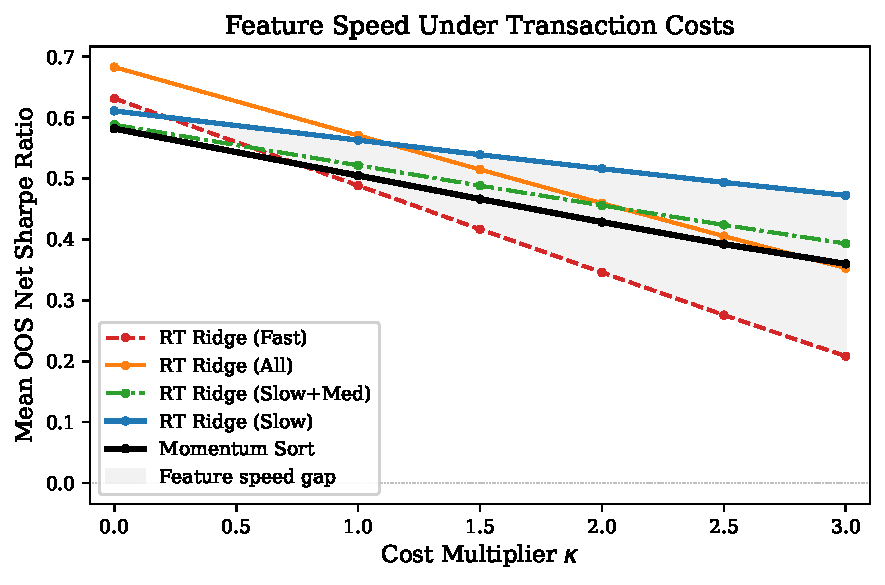
\includegraphics[width=\columnwidth]{figures/cost_speed_crossover.pdf}
\caption{Net SR vs.\ cost multiplier $\kappa$. Fast features degrade
${\sim}3\times$ faster than slow features. The shaded region shows the
feature-speed gap, which widens monotonically with $\kappa$. At zero
costs, fast and slow are competitive; at 3$\times$ EM costs, the gap
exceeds 0.25~SR.}
\label{fig:cost_speed}
\end{figure}

In EM, the cost--speed interaction is 3--5$\times$ larger than in US
markets, suggesting that downstream optimization alone may not
suffice; the problem must also be addressed upstream.


\subsection{ML vs.\ Sorts: Ridge Matches Momentum}
\label{sec:ml_vs_sorts}

With rank-target training, Ridge essentially matches MomentumSort across
15 EM markets at 3$\times$ costs: average net SRs are Blend 0.38,
MomSort 0.36, Ridge 0.35, CompositeSort 0.32, XGBoost 0.17, LightGBM
0.13. Ridge wins 8/15 markets (Wilcoxon $p = 0.45$, not significant);
tree models are significantly worse ($p < 0.01$).

Table~\ref{tab:gross_vs_net} isolates the cost interaction. Ridge
generates a \emph{stronger} gross signal (0.68) than MomSort (0.58),
but 23\% turnover vs.\ 17\% erases the advantage.

\begin{table}[t]
\centering
\caption{Gross vs.\ net Sharpe ratios at 3$\times$ costs, averaged
across 15 EM markets. Ridge has a stronger gross signal but higher
turnover erases the advantage.}
\label{tab:gross_vs_net}
\small
\begin{tabular}{@{}lrrrr@{}}
\toprule
Strategy & Gross SR & Net SR & Turnover & Cost Drag \\
\midrule
MomentumSort  & 0.58 &  0.36  & 17.0\% & $\sim$590 bps \\
Ridge         & 0.68 &  0.35  & 23.3\% & $\sim$700 bps \\
XGBoost       & 0.66 &  0.17  & 36.3\% & $\sim$1{,}100 bps \\
LightGBM      & 0.64 &  0.13  & 38.2\% & $\sim$1{,}160 bps \\
Blend (80/20) & 0.63 &  0.38  & 19.0\% & $\sim$640 bps \\
\bottomrule
\end{tabular}
\end{table}


Per-market results (Table~\ref{tab:main_comparison}) show Ridge wins
8/15 markets, with advantages where turnover is contained (TWN: 0.73
vs.\ 0.51; CHN: 0.23 vs.\ 0.07). Ridge\_Slow
(Section~\ref{sec:slowridge}) is best in 5 markets, positive in 13/15.

\begin{table*}[t]
\centering
\caption{Out-of-sample net Sharpe ratios at 3$\times$ costs across 15
emerging markets. $N$ is the universe size (top stocks by market cap);
$T_{\text{OOS}}$ is the number of out-of-sample months. Bold indicates
the best active strategy per market. EW is the equal-weighted passive
benchmark. Ridge matches MomSort on average (0.35 vs.\ 0.36) but
generates higher turnover (23\% vs 17\%); Ridge\_Slow
(Section~\ref{sec:slowridge}) reaches 0.47 at 10\% turnover.}
\label{tab:main_comparison}
\small
\resizebox{\textwidth}{!}{%
\begin{tabular}{@{}lrcrrrrrrrrrr@{}}
\toprule
Market & $N$ & $T_{\text{OOS}}$ & EW & MomSort & Composite & Ridge & Ridge\_Slow & XGBoost & LightGBM & Blend & TO$_{\text{Mom}}$ & TO$_{\text{Ridge}}$ \\
\midrule
BRA & 100 & 83  & 0.10 &  \textbf{0.08} &$-$0.04 &$-$0.05 &$-$0.06 &$-$0.30 &$-$0.23 &  \textbf{0.08} & 18\% & 30\% \\
CHN & 300 & 78  & 0.24 &  0.07 &  0.13  &  0.23 &  \textbf{0.39} &$-$0.07 &$-$0.17 &  0.08 & 21\% & 23\% \\
GRC & 50 & 78  & 0.64 &  0.43 &  \textbf{0.92}  &  0.73 &  0.74 &  0.64 &  0.50 &  0.49 & 15\% & 19\% \\
IDN & 100 & 80  & 0.29 &  \textbf{0.59} &  0.13  &  0.42 &  0.54 &  0.22 &  0.14 &  0.47 & 17\% & 18\% \\
IND & 200 & 81  & 0.61 &  \textbf{0.63} &  0.29  &  0.37 &  0.58 &  0.09 &$-$0.11 &  0.59 & 16\% & 28\% \\
KOR & 200 & 86  & 0.07 &  0.03 &$-$0.32 &  \textbf{0.07} &  0.07 &$-$0.23 &$-$0.29 & $-$0.04 & 18\% & 15\% \\
MEX & 100 & 93  & 0.46 &  0.25 &  0.40  &  0.18 &  \textbf{0.51} &$-$0.24 &$-$0.32 &  0.23 & 18\% & 27\% \\
MYS & 100 & 90  & 0.23 &  0.39 &  0.14  &  \textbf{0.46} &  0.43 &  0.24 &  0.28 &  \textbf{0.46} & 15\% & 22\% \\
PHL & 100 & 87  & $-$0.02 &  0.01 &  \textbf{0.41}  &  0.10 &  0.16 &$-$0.14 &$-$0.11 &  0.17 & 15\% & 25\% \\
POL & 100 & 69  & 0.53 &  0.55 &  0.60  &  0.57 &  \textbf{0.70} &  0.60 &  0.57 &  0.55 & 17\% & 24\% \\
SAU & 100 & 56  & 1.01 &  1.13 &  0.93  &  0.85 &  1.20 &  0.93 &  0.94 &  \textbf{1.22} & 14\% & 25\% \\
THA & 100 & 84  & $-$0.09 &  0.01 &$-$0.18 &$-$0.05 &$-$0.06 &$-$0.38 &$-$0.43 &  \textbf{0.09} & 17\% & 20\% \\
TUR & 100 & 79  & 0.61 &  0.33 &  \textbf{0.67}  &  0.45 &  0.54 &  0.39 &  0.43 &  0.35 & 18\% & 24\% \\
TWN & 200 & 78  & 0.67 &  0.51 &  0.54  &  0.73 &  \textbf{0.86} &  0.71 &  0.73 &  0.51 & 17\% & 23\% \\
ZAF & 100 & 93  & 0.30 &  0.39 &  0.24  &  0.24 &  \textbf{0.49} &  0.07 &$-$0.02 &  0.48 & 18\% & 28\% \\
\midrule
\textbf{Mean} & -- & 80 & 0.38 & 0.36 & 0.32 & 0.35 & \textbf{0.47} & 0.17 & 0.13 & 0.38 & 17\% & 23\% \\
\bottomrule
\end{tabular}%
}
\end{table*}


\subsection{The Feature-Speed Decomposition}
\label{sec:mechanism}

The cost--speed interaction (Section~\ref{sec:cost_speed}) establishes
that fast features degrade faster under costs. We now decompose
\emph{why} ML preferentially loads on these features and trace the chain
from feature characteristics to portfolio turnover.

Table~\ref{tab:feature_speed} reports three diagnostics. FAST features
represent 25\% of the feature set but receive 43--47\% of model
importance and generate 63\% of month-to-month prediction changes.
Their low rank autocorrelation (0.68 vs.\ 0.97 for SLOW) makes
predictions inherit their instability.

\begin{table}[t]
\centering
\caption{Feature speed decomposition. FAST features dominate both
model importance and prediction changes despite representing a
minority of the feature set.}
\label{tab:feature_speed}
\begin{tabular}{@{}lrrrr@{}}
\toprule
Speed & \# Feat. & Rank AC & \% Import. & \% Pred.\ $\Delta$ \\
\midrule
SLOW   & 57 & 0.97 & 31--34\%  & 12.6\% \\
MEDIUM & 56 & 0.83 & 22--23\%  & 24.1\% \\
FAST   & 38 & 0.68 & 43--47\%  & 63.4\% \\
\bottomrule
\end{tabular}
\end{table}


\paragraph{Feature overweighting.}
FAST features (25\% of the set) receive 43\% of importance in
Ridge and 47\% in XGBoost, drawn by high-frequency signal-to-noise
advantages in the training objective.

\paragraph{Stock-level IC confirms the tradeoff.}
Table~\ref{tab:ic_analysis} quantifies the prediction-stability tradeoff.
Ridge\_Slow achieves the highest IC$\times$stability (0.030), pairing a
momentum-level IC (0.031) with near-perfect stability (0.939);
Ridge\_Fast has the lowest stability (0.539) with no IC compensation,
confirming fast features as the primary instability source.

\begin{table}[t]
\centering
\caption{Information coefficient analysis across 15 EM markets.
IC$\times$Stability captures the effective signal after accounting for
prediction churn.}
\label{tab:ic_analysis}
\begin{tabular}{@{}lrrrr@{}}
\toprule
Strategy & IC & Stability & IC$\times$Stab & Hit Rate \\
\midrule
MomentumSort  & 0.031 & 0.894 & 0.028 & 57.6\% \\
Ridge\_All    & 0.022 & 0.665 & 0.015 & 57.0\% \\
Ridge\_Slow   & 0.031 & 0.939 & \textbf{0.030} & 57.7\% \\
Ridge\_Fast   & 0.013 & 0.539 & 0.007 & 54.0\% \\
\bottomrule
\end{tabular}
\end{table}

\paragraph{Model-free signal decay.}
The speed differential is a data property, not a modeling artifact.
With no fitted model, we compute per-feature monthly rank ICs against
single-month returns at horizons of 1--12 months, sign-aligned per
feature. One-month ICs are comparable (slow 0.027, fast 0.025), but
slow features retain 69\% of their IC at a 12-month horizon versus
57\% for fast features (Wilcoxon $p = 0.01$ across 15 markets;
Figure~\ref{fig:ic_decay}). Notably, fast features' predictive
\emph{content} decays only moderately faster; it is their
\emph{values} that churn (rank AC 0.68 vs.\ 0.97,
Table~\ref{tab:feature_speed}), which is what forces turnover. This
confirms the cost interaction of Section~\ref{sec:cost_speed}: fast
signals remain informative, but trading them is expensive.

\begin{figure}[t]
\centering
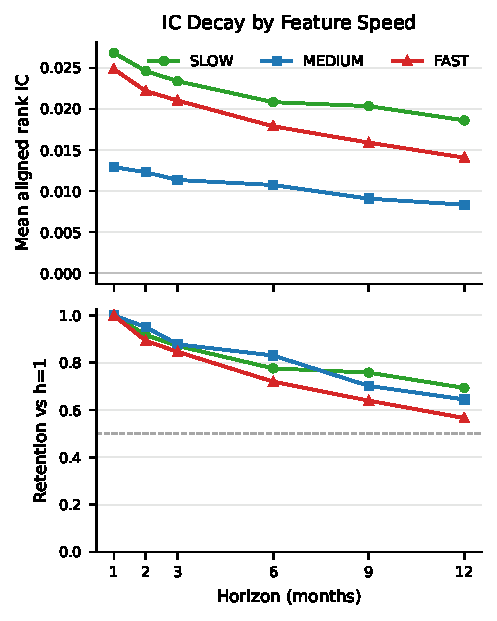
\includegraphics[width=0.8\columnwidth]{figures/ic_decay_by_speed.pdf}
\caption{Model-free rank-IC decay by feature speed class. Slow
features retain 69\% of their one-month IC at 12 months versus 57\%
for fast features; no model is fitted anywhere in this analysis.}
\label{fig:ic_decay}
\end{figure}

\paragraph{Summary.}
FAST features $\xrightarrow{\text{high importance}}$
unstable predictions $\xrightarrow{\text{high turnover}}$
low net SR. This structural tension between predictive power and
tradability produces a modest drag in low-cost environments and
strategy failure in high-cost EM.


\subsection{Upstream Fix: Slow-Feature Ridge}
\label{sec:slowridge}

The decomposition motivates a simple upstream fix: restrict features
to slow, persistent characteristics before training.
Table~\ref{tab:feature_speed_test} confirms this dramatically.
Ridge\_Slow achieves net SR 0.47 at 10\% turnover versus MomSort's
0.36 at 17\%, with the \emph{same model and hyperparameters}. The
improvement comes entirely from removing fast features. (A pooled
block bootstrap yields $p = 0.10$ for the SR difference; see
Section~\ref{sec:robustness}. Ridge\_Slow outperforms in 11/15
markets and 90\% of bootstrap samples; detecting an effect of this
magnitude at 5\% would require ${\sim}$80 years of OOS data.)

\paragraph{Aggregation versus speed.}
Comparing Ridge and CompositeSort at matched dimensionality
($N \in \{5, 10, 20, 50\}$): at $N = 5$, turnover is nearly identical
(5.1\% vs.\ 5.6\%), ruling out regression itself as the turnover
source.

\paragraph{Data-driven persistence filter.}
A persistence filter (rank AC $> 0.75$, recomputed on training data;
${\sim}$120 features) and a speed-tercile split (${\sim}$127 features)
both yield net SR 0.47 at 13\% turnover, matching the ad-hoc result.

\begin{table}[t]
\centering
\caption{Feature-speed ablation: Ridge with different feature
subsets. Mean OOS net SRs across 15 markets at 3$\times$ costs.}
\label{tab:feature_speed_test}
\small
\begin{tabular}{@{}lrrr@{}}
\toprule
Strategy & Net SR & Turnover & \# Features \\
\midrule
\textbf{Ridge\_Slow}   & \textbf{0.47} & \textbf{10.2\%} & 57 \\
Ridge\_SlowMed         & 0.39 & 14.5\% & 113 \\
MomentumSort           & 0.36 & 17.0\% & 1 \\
Ridge\_All             & 0.35 & 23.3\% & 151$^\dagger$ \\
Ridge\_Fast            & 0.21 & 30.1\% & 38 \\
\bottomrule
\multicolumn{4}{@{}l@{}}{\footnotesize $^\dagger$154 characteristics minus \texttt{me} (universe filter), target, and identifier.}
\end{tabular}
\end{table}

This upstream fix requires no cost-aware optimization, no prediction
smoothing, and no change to portfolio construction. It is the simplest
intervention with the largest improvement.

\paragraph{Alpha over the passive benchmark.}
To isolate stock-selection skill, we compute $\text{SR}_\alpha =
\text{SR}(r_p - r_{\text{EW}})$, where $r_{\text{EW}}$ is the
equal-weighted universe return. At 3$\times$ costs: Ridge\_Slow
$\text{SR}_\alpha = +0.18$ (positive in 10/15 markets), MomSort $+0.07$
(8/15), Ridge\_All $-0.15$ (6/15), Ridge\_Fast $-0.46$ (2/15). At
1$\times$ costs, all variants produce comparable positive alpha,
confirming the gap is entirely cost-mediated.


\subsection{Model Complexity Amplifies the Cost Channel}
\label{sec:tree_inversion}

We extend the analysis to tree-based models, revealing a second
mechanism, model complexity, that amplifies the disconnect
independently of feature speed.

Table~\ref{tab:tree_inversion} presents gross-to-net performance across
all model--feature combinations on a common sample. XGBoost achieves
the highest
unsmoothed gross SR (0.77), yet its net SR (0.30) falls well below
Ridge\_All (0.36) and Ridge\_Slow (0.48). The gross ranking is strongly
inverted in net terms (rank correlation $-$0.52 across model--feature
combinations).

\begin{table}[t]
\centering
\caption{The prediction-portfolio disconnect across model classes and
smoothing interventions. Sorted by gross SR. All rows use the
tree-comparison sample: walk-forward over all
months after the initial 60-month training window (${\sim}$102 months
per market), a longer window than Tables~\ref{tab:gross_vs_net}%
--\ref{tab:main_comparison}'s OOS period, so levels are not comparable
across tables.}
\label{tab:tree_inversion}
\small
\begin{tabular}{@{}llrrrr@{}}
\toprule
Model & Strategy & Gross SR & Net SR & SR Lost & TO \\
\midrule
XGB   & All          & 0.767 & 0.300 & $-$0.467 & 34.5\% \\
LGBM  & All          & 0.748 & 0.265 & $-$0.482 & 35.5\% \\
Ridge & All          & 0.684 & 0.357 & $-$0.326 & 23.0\% \\
XGB   & Slow         & 0.647 & 0.263 & $-$0.385 & 28.6\% \\
Ridge & Slow         & 0.616 & 0.479 & $-$0.137 & 9.9\% \\
MomSort & ---        & 0.606 & 0.373 & $-$0.233 & 17.2\% \\
\bottomrule
\end{tabular}
\end{table}

\paragraph{Slow features do not help trees; smoothing only partly
does.}
XGB\_Slow (net SR 0.263) performs \emph{worse} than XGB\_All (0.300),
because decision boundary shifts generate turnover independent of
input stability. Output smoothing is the more effective lever, but
only partially: on the main OOS sample, walk-forward EMA lifts
XGBoost's net SR from 0.24 to 0.35 (turnover 36\% to 25\%),
recovering sort parity (0.36) but not the frontier. Even the best
fixed $\alpha = 0.2$, selected post hoc, reaches 0.45 at 12\%
turnover, approaching but not exceeding Ridge\_Slow's 0.47. A
post-2020 validation had suggested smoothed trees exceed
Ridge\_Slow (0.53); this does not replicate on the full sample.

\paragraph{A $2 \times 2$ framework.}
The results decompose into feature speed $\times$ model smoothness
(Figure~\ref{fig:two_by_two}): Ridge\_Slow loses only 0.14~SR to
costs, Ridge\_All 0.33, XGB\_Slow 0.39, XGB\_All 0.47. Output
smoothing partially bridges the gap (walk-forward EMA cuts
XGBoost's gross-to-net loss from 0.49 to 0.33 on the main OOS
sample),
confirming that prediction instability, not model capacity, is
the mechanism.

\paragraph{Implication.}
The binding constraint is prediction \emph{stability}, not accuracy.
EMA is a universal lever: it improves Ridge (+0.10~SR) and XGBoost
(+0.11 walk-forward, +0.21 post hoc), but cannot fully compensate
for piecewise-constant surfaces. Trees' superior gross signal (0.72
unsmoothed vs.\ 0.61 for Ridge\_Slow on the main OOS sample) is
offset by residual instability, explaining why simple linear models
remain competitive after
costs~\cite{gu2020empirical, esakia2025longonly}.

\begin{figure}[t]
\centering
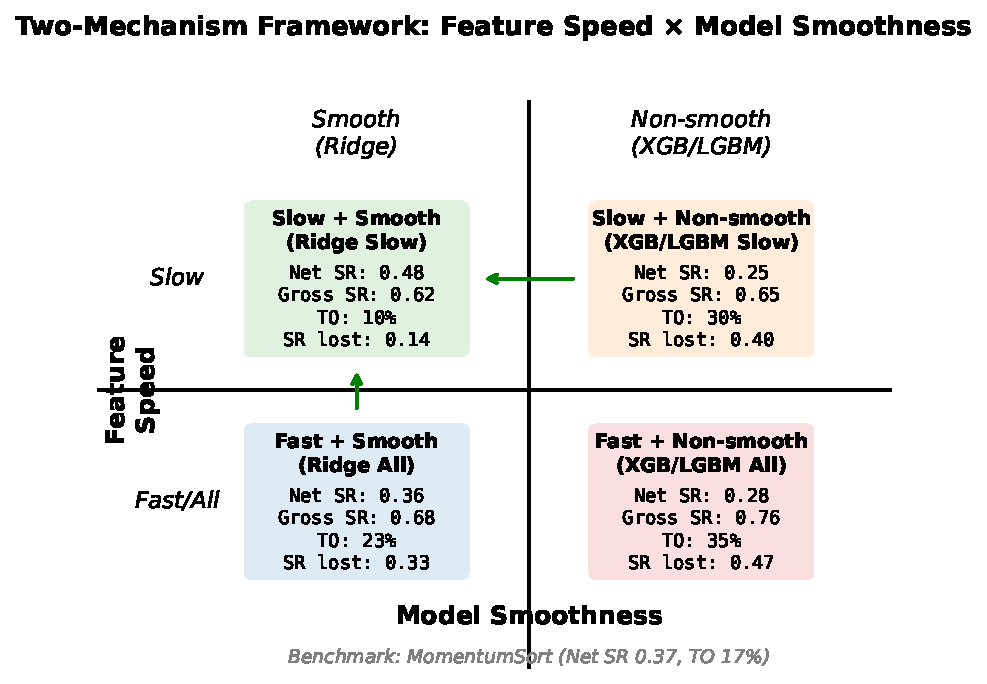
\includegraphics[width=0.85\columnwidth]{figures/two_by_two.pdf}
\caption{The $2 \times 2$ framework: feature speed $\times$ model
smoothness. Both slow features and a smooth model are needed to
minimize the prediction-portfolio disconnect.}
\label{fig:two_by_two}
\end{figure}


\subsection{The Cost-Speed Frontier}
\label{sec:fsi_results}

We estimate the frontier (Equation~\ref{eq:bound}) on smooth models
(Ridge variants, sorts) across 300 strategy--market--cost combinations
(5~strategies $\times$ 15~markets $\times$ 4~cost levels).
Figure~\ref{fig:bound} plots $\kappa \cdot \text{FSI}$ against SR
degradation: pooled $R^2 = 0.72$. Because costs are proportional to
$\kappa$, per-$\kappa$ slopes of $0.33\kappa$ are arithmetic, not
evidence; they confirm only that these strategies trade identically
at every cost level. The substantive result is cross-sectional: at
each fixed $\kappa$, FSI alone explains 64--65\% of degradation
across the 75 strategy--market cells ($\kappa$ alone: 37\% pooled).
We quote the per-$\kappa$ slope $\lambda = 0.33$ throughout (the
pooled slope, 0.39, overweights high-$\kappa$ cells; cluster-robust
95\% CIs: $[0.27, 0.40]$ by market, $[0.26, 0.41]$ by strategy). FSI
is equally an ex-ante turnover diagnostic (it explains 73\% of
realized turnover across cells) and is computable from training data
\emph{before} any trading occurs. Its resolution is at the strategy
level: FSI is a feature-set property, nearly constant across markets
within a strategy, so it separates feature sets rather than markets
(within-strategy $R^2 = 0.07$); its coefficient is unchanged when
controlling for each market's spread level.

Pooling tree models (XGBoost, LightGBM; same OOS window as
Table~\ref{tab:gross_vs_net}) with a non-smoothness indicator turns
the second channel into a joint test rather than a residual
description: at $\kappa = 3$, $R^2$ rises from 0.34 to 0.73 with
$+$0.22~SR excess tree degradation and an unchanged FSI coefficient.
EMA output smoothing moves trees toward the frontier without
reaching it (walk-forward: 0.24 to 0.35; best post-hoc fixed
$\alpha$: 0.45 at 12\%~TO).

Figure~\ref{fig:frontier} visualizes the resulting frontier. At 3$\times$
EM costs, eight strategies cluster near net SR 0.45--0.49 despite
radically different mechanisms: slow-feature selection (Ridge\_Slow
0.47), persistence filtering (0.47), speed-tercile selection (0.47),
a data-driven rank-target variant (0.46), fixed and walk-forward EMA
smoothing (0.47 and 0.45), and quarterly rebalancing (Ridge\_All\_Q
0.48, Ridge\_Slow\_Q 0.49). Strategies that fail to minimize FSI (tree models,
fast-feature Ridge, unconstrained NNs) fall below the ceiling in
proportion to $\kappa \cdot \text{FSI}$.

The ceiling height depends on $\text{SR}_{\text{gross}}$ and the
market's cost environment; the frontier's portable content is the
cross-sectional FSI--degradation relationship at each cost level.

\begin{figure}[t]
\centering
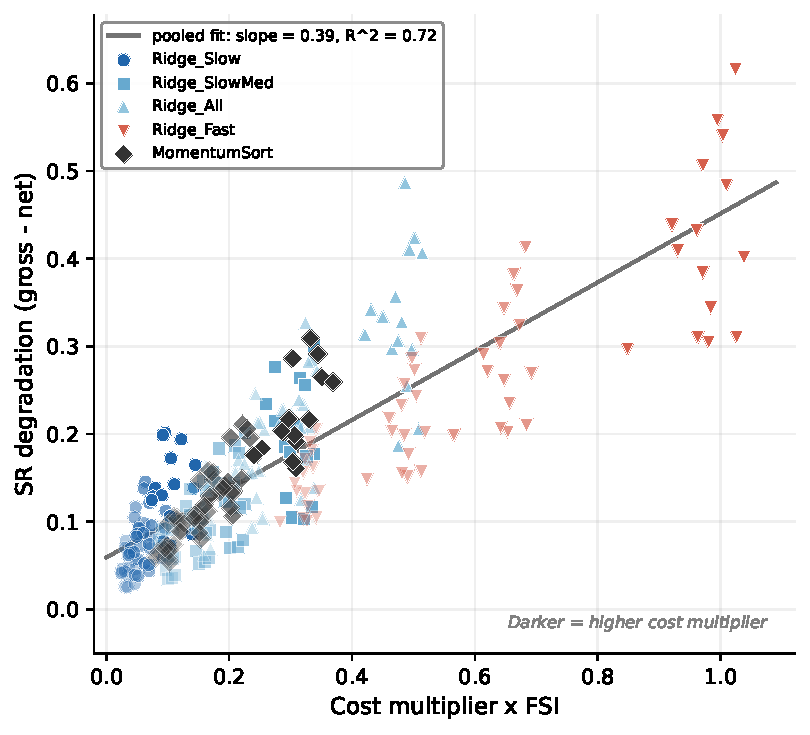
\includegraphics[width=\columnwidth]{figures/cost_speed_bound.pdf}
\caption{The cost-speed frontier (Equation~\ref{eq:bound}): SR
degradation vs.\ $\kappa \times \text{FSI}$ across 300
strategy--market--cost combinations. Pooled $R^2 = 0.72$;
cross-sectional $R^2 = 0.64$--$0.65$ at each fixed $\kappa$ with
slope $\lambda = 0.33$ per unit $\kappa$. Darker points indicate
higher $\kappa$.}
\label{fig:bound}
\end{figure}

\begin{figure}[t]
\centering
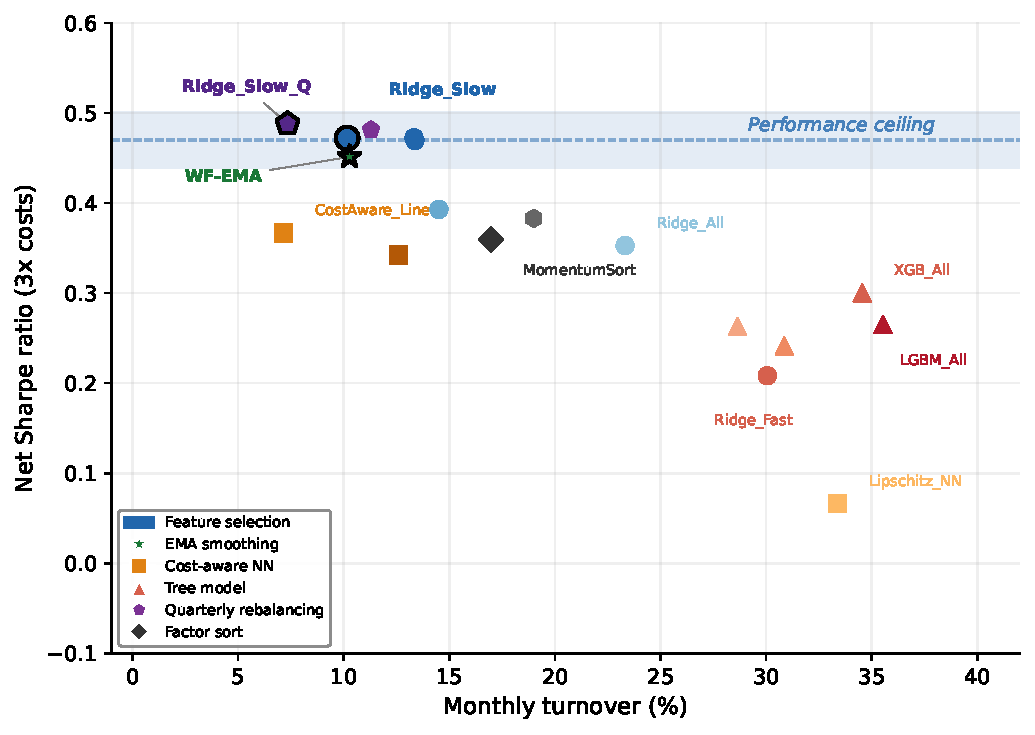
\includegraphics[width=\columnwidth]{figures/cost_speed_frontier.pdf}
\caption{The cost-speed frontier at 3$\times$ EM costs. Strategies
that minimize FSI converge on net SR ${\sim}$0.45--0.49 (shaded
band). Below the ceiling, net SR degrades with turnover along the
frontier. Color indicates mechanism type.}
\label{fig:frontier}
\end{figure}

\paragraph{Cross-market transfer.}
To test whether the frontier generalizes out of sample, we run
leave-one-market-out (LOMO) and leave-5-out cross-validation. LOMO
(15~folds) yields mean OOS $R^2 = 0.60$; leave-5-out (3{,}003~splits)
yields mean OOS $R^2 = 0.69$, with 97\% of splits above 0.50.
The fitted slope is stable across folds (std $= 0.008$, range
$[0.37, 0.40]$; bootstrap 95\% CI $[0.34, 0.45]$), so the
cross-sectional relationship is not driven by any single market. The
slow-feature set also transfers: 52 of 57 slow features are classified
as slow in \emph{all} 15 markets (mean Jaccard similarity 0.97), so
``slow'' can be defined on one market subset and applied elsewhere.


\subsection{Prediction Smoothing}
\label{sec:smoothing}

A complementary intervention smooths predictions at the output level.
We apply an EMA to Ridge's prediction ranks:
$\hat{r}_{i,t}^{\text{smooth}} = \alpha \cdot \hat{r}_{i,t}^{\text{raw}}
+ (1 - \alpha) \cdot \hat{r}_{i,t-1}^{\text{smooth}}$,
where lower $\alpha$ means more smoothing. Figure~\ref{fig:ema_curve}
shows the alpha--SR relationship. The curve peaks at $\alpha = 0.35$
(net SR 0.47), forming an inverted-U. Walk-forward alpha
selection, maximizing IS net SR over the last 24 training
months scored by the current-window model, achieves 0.45 without using
future OOS months, beating MomSort (0.36) in 10/15 markets.

\begin{figure}[t]
\centering
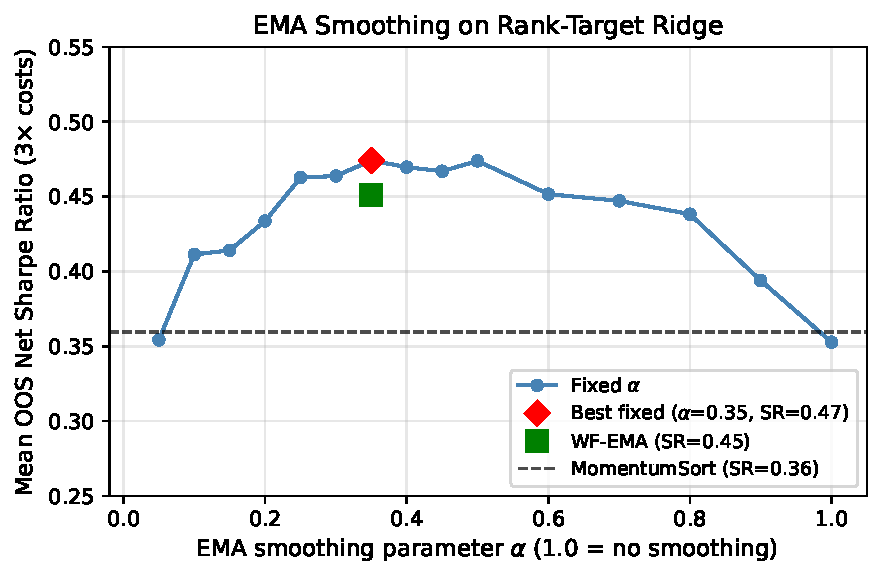
\includegraphics[width=0.85\columnwidth]{figures/ema_alpha_curve.pdf}
\caption{EMA smoothing: $\alpha$ vs.\ net SR at 3$\times$ costs
(15 markets). Walk-forward EMA (green square) achieves 0.45,
beating MomSort (0.36).}
\label{fig:ema_curve}
\end{figure}

Table~\ref{tab:ema_results} quantifies the gains. WF-EMA's gross SR
(0.60) is \emph{below} unsmoothed Ridge (0.68): the +0.10 net SR
improvement comes entirely from turnover reduction (23\% $\to$ 10\%).
EMA helps Ridge but \emph{hurts} MomSort ($-$0.04), confirming it
recovers ML-specific signal.

\begin{table}[t]
\centering
\caption{Prediction smoothing results (15 markets). WF-EMA selects
$\alpha$ inside the walk-forward loop using recent in-sample months and
does not use future OOS months.}
\label{tab:ema_results}
\small
\begin{tabular}{@{}lrrrrr@{}}
\toprule
Strategy & Net SR & Gross SR & TO & Stability & Wins \\
\midrule
Ridge (no smooth)   & 0.35 & 0.68 & 23.3\% & 0.750 & 8/15 \\
MomentumSort        & 0.36 & 0.58 & 17.0\% & ---   & --- \\
\textbf{Ridge WF-EMA} & \textbf{0.45} & \textbf{0.60} & \textbf{10.3\%} & \textbf{0.919} & \textbf{10/15} \\
\bottomrule
\end{tabular}
\end{table}

\paragraph{EMA is redundant with slow features.}
Ridge\_Slow with EMA selects $\alpha = 1.0$ (no smoothing): when
features are already slow, predictions are inherently stable
(rank stability 0.939, Table~\ref{tab:ic_analysis}). The two
interventions are substitutes.

\paragraph{EMA helps tree models, but less reliably.}
EMA is not Ridge-specific: it lifts XGBoost from 0.24 to 0.35
(Section~\ref{sec:tree_inversion}). Two differences from Ridge: the
optimal smoothing is more aggressive ($\alpha = 0.2$ vs.\ 0.35),
reflecting trees' greater inherent instability, and walk-forward
selection captures barely half the post-hoc gain (+0.11 of +0.21;
Ridge captures +0.10 of +0.12), because trees' noisier in-sample
net SR misguides the $\alpha$ choice.


\subsection{Cross-Regime Validation: US Equities}
\label{sec:us_validation}

We test the identical pipeline on US equities (top 500 by market cap,
OOS 2021--2025, 50 months). Table~\ref{tab:us_validation} confirms
the decomposition is not EM-specific: Ridge\_Slow outperforms Ridge\_Fast
at every cost level, and Ridge\_Fast collapses at 3$\times$ costs
($-$0.19 vs.\ 0.51). MomentumSort retains a clear advantage in the
US; we do not claim Ridge beats
MomSort there. The EM--US divergence reflects two channels:
MomSort's gross signal is substantially stronger in the US (0.78 vs.\
0.58 in EM), and EM costs are 3--5$\times$ larger, making the turnover
reduction from slow-feature selection more valuable relative to the
sort's advantage. The key point is that the \emph{relative} patterns
within Ridge's feature subsets replicate precisely.

\begin{table}[t]
\centering
\caption{US equities: net SR by strategy and cost multiplier. Top 500,
OOS 2021--2025. Ridge\_Slow outperforms Ridge\_Fast at every cost
level; Ridge\_Fast goes negative at 3$\times$.}
\label{tab:us_validation}
\small
\begin{tabular}{@{}lrrrr@{}}
\toprule
$\kappa$ & MomSort & Ridge\_All & Ridge\_Slow & Ridge\_Fast \\
\midrule
0$\times$ & 0.775 & 0.580 & 0.638 & 0.404 \\
1$\times$ & 0.693 & 0.445 & 0.574 & 0.206 \\
2$\times$ & 0.612 & 0.310 & 0.510 & 0.008 \\
3$\times$ & 0.530 & 0.175 & 0.510 & $-$0.189 \\
\bottomrule
\end{tabular}
\end{table}

\paragraph{Two channels.}
The decomposition operates through signal degradation and cost
amplification. Ridge\_Fast trails Ridge\_Slow even at zero costs
(0.40 vs.\ 0.64), and the gap widens from 0.23 to 0.70~SR as
$\kappa$ rises from 0 to 3. In EM, ML concentrates importance on fast
features well beyond their share of the feature set
(Table~\ref{tab:feature_speed}), compounding both channels.


%% ===================================================================
%% 5. DISCUSSION
%% ===================================================================
\section{Discussion}

\paragraph{Theoretical foundation: GP, JKMP, and the ceiling.}
Our cost-speed frontier (Equation~\ref{eq:bound}) operationalizes
G\^{a}rleanu and Pedersen's~\cite{garleanu2013dynamic} (GP) insight
that optimal portfolios overweight slow-decaying signals. GP prove this
in continuous time with known dynamics; we show the same structure
creates a quantifiable ceiling in a discrete-time ML pipeline with
154 estimated characteristics. A per-$\kappa$ slope of exactly
$\lambda\kappa$ under proportional costs means strategies trade
identically at every cost level. This is a diagnosis, not a discovery:
cost-aware strategies (JKMP-style) would cut turnover as $\kappa$
rises, bending the frontier ($\lambda$ decreasing in $\kappa$).
Standard ML pipelines show no such adaptation, motivating the
upstream fix.
JKMP~\cite{jensen2024implementable} optimize downstream (cost-aware
training); we characterize the ceiling that any method, upstream or
downstream, approaches. In EM, where cost estimates are noisy, the
upstream fix reaches the ceiling without requiring reliable cost
inputs.

The $2 \times 2$ framework (Section~\ref{sec:tree_inversion}) reveals
why non-smooth models cannot reach the ceiling: model smoothness is a
second constraint that feature selection alone cannot address. On the
same slow features, trees and unconstrained NNs exhibit excess
degradation correlated $r = 0.91$ with model-induced turnover.
Both slow inputs \emph{and} smooth models are needed.

\paragraph{Reconciling with Hanauer and Kalsbach.}
Hanauer and Kalsbach~\cite{hanauer2023machine} show ML produces superior
long-short Sharpe ratios vs.\ linear models in EM. We confirm their
core finding: ML generates stronger \emph{gross} signals (Ridge gross
SR 0.68 vs.\ MomSort 0.58). The divergence arises from the evaluation
framework: we benchmark against factor sorts (sparse, low-turnover,
and thus a harder cost-adjusted benchmark); we evaluate long-only
portfolios, since short-selling is restricted in most EM
(Section~\ref{sec:robustness}); and at
realistic EM costs ($\kappa = 3$, $\sim$90~bps one-way), ML's turnover
from fast-feature loading erases the signal advantage. Our results
complement rather than contradict Hanauer: they identify the
implementation boundary beyond which ML's signal superiority no longer
translates to portfolio outperformance.

\paragraph{Practical recommendations.}
For EM equity portfolios: (1)~without ML infrastructure, default to
momentum sorts; (2)~teams with ML should restrict to
slow features and train on rank targets, which beats the sort without
prediction smoothing or cost-aware optimization. In our data, fast features'
gross advantage survives only below $\kappa \approx 0.2$
(${\sim}$6~bps one-way): at all realistic EM cost levels, slow
features dominate.
The FSI provides an ex-ante screen: compute Equation~\ref{eq:fsi} before
deployment, and if FSI exceeds $\sim$0.15, restrict features or apply
smoothing.

\paragraph{Limitations.}
Our OOS spans 56--93 months per market with cross-country correlation
${\sim}$0.6, limiting statistical power (see
Section~\ref{sec:robustness} for formal tests). The Corwin-Schultz
cost model with 3$\times$ multiplier is validated against an EM equity
fund but remains a proxy. We test only large-caps; ML may fare better
in small-caps, but costs there are higher. Tree hyperparameters are
fixed at standard values~\cite{gu2020empirical}, making our comparison
conservative. Implementation choices affect
results~\cite{chen2025nonstandard}, though the feature-speed
decomposition reflects data properties rather than modeling choices.
Combining upstream feature selection with JKMP-style downstream
optimization is untested.


%% ===================================================================
%% 6. ROBUSTNESS
%% ===================================================================
\section{Robustness and Alternatives}
\label{sec:robustness}

\paragraph{Cost-aware neural networks.}
Cost-aware training objectives could address turnover without
discarding features. We test three alternatives, \emph{all restricted
to the 57 slow features}: (i)~\textbf{CostAware\_\allowbreak Linear} (linear model
with differentiable net-of-cost Sharpe loss),
(ii)~\textbf{CostAware\_\allowbreak Lipschitz} (spectral-norm MLP with cost
penalty), and (iii)~\textbf{Lipschitz\_\allowbreak NN} (spectral-norm MLP without
cost penalty), all with rank targets and walk-forward HP selection.
Ridge\_Slow remains best (Table~\ref{tab:cost_aware_nn}).
CostAware\_Linear achieves 7.1\% turnover but sacrifices gross signal
(net SR 0.37). Lipschitz\_NN fails entirely (SR 0.07, 33\% turnover):
even with slow inputs, the nonlinear prediction surface generates
instability. Coupling signal and turnover in a single loss forces a
tradeoff that the simple upstream fix avoids.

\begin{table}[t]
\centering
\caption{Cost-aware alternatives vs.\ Ridge\_Slow (rank targets).
Mean OOS across 15 markets at 3$\times$ costs. No cost-aware
variant matches the upstream fix.}
\label{tab:cost_aware_nn}
\small
\begin{tabular}{@{}lrrr@{}}
\toprule
Strategy & Net SR & Turnover & Gross SR \\
\midrule
\textbf{Ridge\_Slow}        & \textbf{0.47} & 10.2\% & 0.61 \\
CostAware\_Linear   & 0.37 & 7.1\%  & 0.47 \\
MomentumSort        & 0.36 & 17.0\% & 0.58 \\
CostAware\_Lipschitz & 0.34 & 12.6\% & 0.52 \\
Lipschitz\_NN       & 0.07 & 33.4\% & 0.48 \\
\bottomrule
\end{tabular}
\end{table}

\paragraph{Long-short portfolios.}
Short-selling is restricted or prohibitively expensive in most EM.
On five markets (BRA, IND, KOR, TWN, THA) at 3$\times$ costs plus
50~bps borrowing cost, short-only net SRs are negative for
\emph{every} strategy (MomSort $-$0.44, Ridge $-$0.76, XGBoost
$-$0.98): the short leg's 19--58\% turnover overwhelms any signal,
reinforcing long-only as the relevant EM evaluation.

\paragraph{Quarterly rebalancing.}
Quarterly rebalancing lifts Ridge\_All from 0.35 to 0.48 at 11\%
turnover, matching Ridge\_Slow (0.47, 10\%) with no feature
selection at all; Ridge\_Slow\_Q reaches 0.49 at 7\% and
MomentumSort\_Q barely changes (0.37). We do not discount this: it is
what the frontier predicts (trading a third as often shrinks turnover
regardless of signal mix), and it confirms the ceiling is
mechanism-agnostic. The two routes are performance-equivalent in our
sample but differ operationally: slow-feature selection retains
monthly reactivity and an ex-ante diagnostic, while quarterly
rebalancing holds stale fast-feature positions for three months and
is validated only ex post. Stacking both adds little (0.49),
consistent with substitutes on the same frontier.

\paragraph{Statistical significance.}
Jobson-Korkie tests with the Memmel~\cite{memmel2003performance}
correction are significant at 5\% in no individual market for
MomSort~$>$~Ridge (aggregate Wilcoxon $p = 0.45$) or
MomSort~$>$~XGBoost ($p = 0.008$), and in 1/15 markets for
MomSort~$>$~LightGBM ($p = 0.003$); individual markets lack power at
56--93 OOS months.
For Ridge\_Slow vs.\ MomSort, we pool monthly net returns across all
15 markets and apply a block bootstrap (10{,}000 replications,
resampling dates to preserve cross-market dependence): one-sided
$p = 0.10$, 95\% CI $[-0.08,\; 0.51]$ for the annualized SR
difference. Ridge\_Slow outperforms in 90\% of bootstrap samples and
11/15 markets; a $t$-test on pooled monthly differences gives
$t = 0.77$ ($p = 0.22$). The effect size ($d = 0.08$) would require
${\sim}$980 months of OOS data for 80\% power at $\alpha = 0.05$: no
feasible test can detect an improvement of this magnitude at
conventional levels.
The frontier claim is, however, jointly testable: sign-flipping the
eight interventions' per-market SR differences vs.\ MomentumSort at
the market level ($2^{15}$ exact patterns) gives mean $+0.11$,
$p = 0.008$ (Wilcoxon 0.015). Since the eight variants span four
mechanism families and markets are correlated, we read this as
consistent joint evidence, not eight independent confirmations.
Excluding
the smallest universe (GRC, $N = 50$) leaves the hierarchy intact
(Ridge\_Slow 0.45 vs.\ MomSort 0.36; band 0.42--0.47), as does
value-weighted construction (Ridge\_Slow 0.40 vs.\ MomSort 0.31,
Ridge\_All 0.30; wins 10/15, positive 14/15).

\paragraph{Feature classification sensitivity.}
A data-driven persistence filter (rank AC $> 0.75$; ${\sim}$120
features) and a speed-tercile split (${\sim}$127 features) both yield
net SR 0.47 at 13\% turnover, matching the ad-hoc classification
despite retaining $2\times$ as many features.


%% ===================================================================
%% 7. CONCLUSION
%% ===================================================================
\section{Conclusion}

We show that ML equity strategies in emerging markets face a
cost-speed ceiling: across 15 markets and eight intervention
variants, net Sharpe ratios converge on ${\sim}$0.45--0.49 at
3$\times$ EM transaction costs. The ceiling is traced by a linear
frontier (Equation~\ref{eq:bound}): at each fixed cost level, the
ex-ante Feature Speed Index explains 64--65\% of cross-sectional SR
degradation ($\lambda = 0.33$ per unit $\kappa$; pooled $R^2 = 0.72$)
and 73\% of realized turnover. Non-smooth models (trees and
unconstrained NNs) fall systematically below the frontier, confirming
model smoothness as an independent cost channel.

The frontier implies that the problem is \emph{not} which intervention to
choose, but whether a strategy minimizes its Feature Speed Index.
Feature selection, prediction smoothing, and reduced rebalancing
frequency all reach the same ceiling through different mechanisms.
Restricting Ridge to slow features is the simplest path (SR 0.47, 10\%
turnover); walk-forward EMA independently achieves 0.45.

Model complexity introduces a second constraint: tree models require
output smoothing (EMA) to reach the ceiling, because piecewise-constant
surfaces generate turnover independent of input stability.

More broadly,
the ceiling validates G\^{a}rleanu and
Pedersen's~\cite{garleanu2013dynamic} prediction that optimal
portfolios overweight slow signals, and quantifies the frontier that
any practical ML strategy must respect.


%% ===================================================================
%% ACKNOWLEDGMENTS
%% ===================================================================
\begin{acks}
[Removed for anonymous review.]
\end{acks}


%% ===================================================================
%% REFERENCES
%% ===================================================================
\bibliographystyle{ACM-Reference-Format}
\bibliography{references}


\end{document}
